%!TEX root = ../../book_ML.tex
\chapter{Ôn tập Xác suất}
\label{cha:prob}
%  -- -
% \textbf{Trong trang này:}


% - \href{http://machinelearningcoban.com#-gioi-thieu}{1. Giới thiệu}
% - \href{http://machinelearningcoban.com#-xac-suat}{2. Xác Suất}
%   - \href{http://machinelearningcoban.com#-random-variables}{2.1. Random variables}
%   - \href{http://machinelearningcoban.com#-joint-probability}{2.2. Joint probability}
%   - \href{http://machinelearningcoban.com#-marginalization}{2.3. Marginalization}
%   - \href{http://machinelearningcoban.com#-conditional-probability}{2.4. Conditional probability}
%   - \href{http://machinelearningcoban.com#-quy-tac-bayes}{2.5. Quy tắc Bayes}
%   - \href{http://machinelearningcoban.com#-independence}{2.6. Independence}
%   - \href{http://machinelearningcoban.com#-ky-vong}{2.7. Kỳ vọng}
% - \href{http://machinelearningcoban.com#-mot-vai-xac-suat-thuong-gap}{3. Một vài xác suất thường gặp}
%   - \href{http://machinelearningcoban.com#-bernouli-distribution}{3.1. Bernoulli distribution}
%   - \href{http://machinelearningcoban.com#-categorical-distribution}{3.2. categorical distribution}
%   - \href{http://machinelearningcoban.com#-univariate-normal-distribution-phan-phoi-chuan-mot-bien}{3.3. Univariate normal distribution $Phân phối chuẩn một biến$}
%   - \href{http://machinelearningcoban.com#-multivariate-normal-distribution}{3.4. Multivariate normal distribution}
%   - \href{http://machinelearningcoban.com#-beta-distribution}{3.5. Beta distribution}
%   - \href{http://machinelearningcoban.com#-dirichlet-distribution}{3.6. Dirichlet distribution}
% - \href{http://machinelearningcoban.com#-thao-luan}{4. Thảo luận}
% - \href{http://machinelearningcoban.com#-tai-lieu-tham-khao}{5. Tài liệu tham khảo}



% \section{Giới thiệu}

% Cho tới thời điểm này, kế hoạch viết về phần Machine Learning cơ bản của tôi đã thực hiện được 1 nửa. Trong nửa đầu của blog, các bạn đã làm quen (lại) rất nhiều với Đại số tuyến tính và Tối ưu.

% Nhìn chung, tôi đều viết các thuật toán Machine Learning dưới dạng các bài toán tối ưu và cách giải mỗi bài toán đó.

% Các bài viết trong nửa đầu có thể chia thành các Phần:

% 1. Bài 1-6: Làm quen với Machine Learning. Một vài thuật toán Machine Learning cơ bản chưa cần nhiều tới tối ưu.

% 2. Bài 7-8: Gradient Descent. Thuật toán tối ưu đơn giản mà hiệu quả cho các bài toán tối ưu không ràng buộc.

% 3. Bài 9-15: Neural Networks. Phần này giúp các bạn nắm được các thành phần cơ bản của một Neural Network và các Networks cơ bản nhất, chủ yếu cho các bài toán classification. Các bài toán tối ưu đều là không ràng buộc, các hàm mất mát hầu hết là không lồi, nghiệm tìm được là các local optimal.

% 4. Bài 16-18: Convex Optimization. Phần này bắt đầu sâu hơn một chút về Tối ưu. Định nghĩa về tập lồi, hàm lồi, bài toán tối ưu lồi và bài toán đối ngẫu. Đây là nền tảng cho rất nhiều thuật toán cơ bản Machine Learning sau này.

% 5. Bài 19-22: Support Vector Machine. Đây là một trong những thuật toán đẹp nhất và 'intuitive' nhất trong Machine Learning. Nếu bạn vào wiki tìm 'Machine Learning' thì sẽ thấy hình đại diện chính là SVM và Kernel SVM. Một trong những điều lý thú của SVM là bài toán tối ưu là lồi và nghiệm tìm được là duy nhất, cũng là global optimal.

% 6. Bài 23-25: Recommendation Systems. Đây là một lớp các bài toán thực tế và quan trọng của Machine Learning. Tôi chủ động thêm phần này vào vì làm giảm lượng toán đã đề cập quá nhiều trong Phần 4 và 5. Các thuật toán và bài toán trong phần này khá đơn giản nhưng kết quả khá tốt.

% 7. Bài 26-29: Dimensionality Reduction. Phần này cũng rất quan trọng trong Machine Learning. PCA gần như được dùng trong hầu hết các bài toán ML, trong khi LDA hiệu quả trong các bài toán classification. SVD, sau này các bạn sẽ thấy, được dùng rất nhiều vì những tính chất đẹp của nó.

% Trong nửa còn lại, tôi sẽ đi vào một mảng lớn khác của ML trong đó các kiến thức về xác suất thống kê được áp dụng rất nhiều, tôi tạm gọi phần này là Bayesian Machine Learning. Các bạn sẽ từ từ được ôn lại kiến thức về Xác Suất Thống Kê và làm quen với các thuật toán Machine Learning cơ bản khác.

% Trong bài viết này, tôi sẽ ôn tập lại những kiến thức về Xác Suất thường được sử dụng trong Machine Learning. Mục 2 sẽ nhắc lại về biến ngẫu nhiên, xác suất đồng thời, xác suất biên, xác suất có điều kiện, và quy tắc Bayes. Mục 3 sẽ nhác lại một vài phân bố xác suất thường dùng.

{Chương này được viết dựa trên Chương 2 và 3 của cuốn \textit{Computer Vision:  Models, Learning, and Inference -- Simon J.D. Prince} (\url{https://goo.gl/GTEXzd}).}

\section{Xác suất}


\subsection{Biến ngẫu nhiên}
\index{biến ngẫu nhiên -- random variable}
\index{random variable -- biến ngẫu nhiên}
\index{phân phối xác suất -- probability distribution}
\index{probability distribution -- phân phối xác suất}
% \index{random variable!}

Một \textit{biến ngẫu nhiên} (random variable) $x$ là một biến dùng để đo những đại lượng không
xác định. Biến này có thể được dùng để ký hiệu kết quả/đầu ra của một thí
nghiệm, ví dụ như tung đồng xu, hoặc một đại lượng biến đổi trong tự nhiên, ví
dụ như nhiệt độ trong ngày. Nếu quan sát một số lượng lớn đầu ra
$\{x_i\}_{i=1}^I$ của các thí nghiệm này, ta có thể nhận được những giá trị khác
nhau ở mỗi thí nghiệm. Tuy nhiên, sẽ có những giá trị xảy ra nhiều lần hơn những
giá trị khác, hoặc xảy ra gần một giá trị này hơn những giá trị khác. Thông tin
về đầu ra này được đo bởi một \textit{phân phối xác suất} (probability distribution) được biểu diễn bằng
một hàm $p(x)$. Một biến ngẫu nhiên có thể là {rời rạc} hoặc {liên
tục}.

Một biến ngẫu nhiên rời rạc sẽ lấy giá trị trong một tập hợp các điểm rời rạc
cho trước. Ví dụ tung đồng xu thì có hai khả năng là \textit{xấp} và
\textit{ngửa}. Tập các giá trị này có thể có thứ tự như khi tung xúc xắc hoặc
không có thứ tự như khi đầu ra là các giá trị \textit{nắng}, \textit{mưa},
\textit{bão}. Mỗi đầu ra có một giá trị xác suất tương ứng với nó. Các giá trị
xác suất này không âm và có tổng bằng một.
\begin{equation}
\label{eqn:30_1}
\text{Nếu}~ x ~\text{là biến ngẫu nhiên rời rạc thì}\quad \sum_{x} p(x) = 1.
\end{equation}
Biến ngẫu nhiên liên tục lấy giá trị là các số thực. Những giá trị này có thể là
hữu hạn, ví dụ thời gian làm bài của mỗi thí sinh trong một bài thi 180 phút,
hoặc vô hạn, ví dụ thời gian phải chờ tới khách hàng tiếp theo. Không như biến
ngẫu nhiên rời rạc, xác suất để đầu ra bằng {chính xác} một giá trị nào đó theo
lý thuyết là bằng không. Thay vào đó, phân phối của biến ngẫu nhiên rời rạc
thường được xác định dựa trên xác suất để đầu ra rơi vào một khoảng giá trị nào
đó. Việc này được mô tả bởi một hàm số được gọi là \textit{hàm mật độ xác suất} (probability density function, pdf). Hàm mật độ xác suất
luôn cho giá trị dương, và tích phân của nó trên toàn miền giá trị đầu ra phải
bằng một.
\index{hàm mật độ xác suất -- probability density function}
\index{probability density function -- hàm mật độ xác suất}
\index{pdf}
\begin{equation}
\label{eqn:30_2}
\text{Nếu}~ x ~\text{là biến ngẫu nhiên liên tục thì} \int p(x)dx = 1.
\end{equation}
% Để giảm thiểu ký hiệu, hàm mật độ xác suất của một biến ngẫu nhiên liên tục
% $x$ cũng được ký hiệu là $p(x)$.

\begin{mynote}
Nếu $x$ là một biến ngẫu nhiên rời rạc thì $p(x) \leq 1,~\forall x$. Trong khi
đó, nếu $x$ là biến ngẫu nhiên liên tục, $p(x)$ có thể nhận giá trị không âm
bất kỳ, điều này vẫn đảm bảo tích phân của hàm mật độ xác suất theo toàn
bộ giá trị của $x$ bằng một.    % Với biến ngẫu nhiên rời rạc, $p(x)$ được
% hiểu là \textit{mật độ xác suất} tại $x$.
\end{mynote}


\subsection{Xác suất đồng thời}
\index{xác suất đồng thời -- joint probability}
\index{joint probability -- xác suất đồng thời}
% \subsection{Joint probability}
Nếu quan sát số lượng lớn các cặp đầu ra của hai biến ngẫu nhiên $x$ và $y$ thì
có những cặp đầu ra xảy ra thường xuyên hơn những cặp khác. Thông tin này được
biểu diễn bằng một phân phối được gọi là \textit{xác suất đồng thời} (joint probability) của $x$ và
$y$, được ký hiệu là $p(x, y)$. Hai biến ngẫu nhiên $x$ và $y$ có thể cùng là
biến ngẫu nhiên rời rạc, liên tục, hoặc một rời rạc, một liên tục. Luôn nhớ rằng
tổng các xác suất trên mọi cặp giá trị $(x, y)$ đều bằng một.
\begin{align}
\text{Cả $x$ và $y$ là rời rạc:}  & &\sum_{x, y} p(x, y) &= 1. \\\
\text{Cả $x$ và $y$ là liên tục:} & &\int p(x, y) dx dy &=1.\\\
x ~\text{rời rạc}, ~ y ~\text{liên tục:} & &\sum_{x} \int p(x, y) dy &= \int \left(\sum_{x} p(x, y) \right)dy = 1.
\end{align}
Xét ví dụ trong Hình \ref{fig:30_1}, phần ``Xác suất đồng thời''. Biến ngẫu nhiên
$x$ thể hiện điểm thi môn Toán của học sinh ở một trường THPT trong một kỳ thi
quốc gia, biến ngẫu nhiên $y$ thể hiện điểm thi môn Vật Lý cũng trong kỳ thi đó.
Đại lượng $p(x = x^*, y = y^*)$ là tỉ lệ giữa tần suất số học sinh được
\textit{đồng thời} $x^*$ điểm môn Toán và $y^*$ điểm môn Vật lý với
toàn bộ số học sinh của trường đó. Tỉ lệ này có thể coi là xác suất khi số học
sinh trong trường là lớn. Ở đây $x^*$ và $y^*$ là các số xác định. Thông thường,
xác suất này được viết gọn lại thành $p(x^*, y^*)$, và $p(x, y)$ được dùng như
một hàm tổng quát để mô tả các xác suất.

Giả sử thêm rằng điểm các môn là các số tự nhiên từ 1 đến 10.

Các ô vuông màu đen thể hiện xác suất $p(x, y)$, với diện tích ô vuông càng lớn
biểu thị xác suất càng cao. Chú ý rằng tổng các xác suất này bằng một.

{Có thể thấy rằng xác suất để một học sinh được 10 điểm môn Toán
và 1 điểm môn Lý rất thấp, điều tương tự xảy ra với 10 điểm môn Lý và 1 điểm môn
Toán. Xác suất để một học sinh được khoảng 7 điểm cả hai môn là cao
nhất.}

% <hr>
% <div class="imgcap">
% <img src ="/assets/30_prob/joint.png" align = "center" width = "800">
% </div>

% <br>
% <div  class = "thecap" style = "text-align: justify" >Hình 1: Joint probability (phần trung tâm có nền mùa lục nhạt), Marginalization (phía trên và bên trái) và Conditional probability (phía dưới và bên phải).</div>
% <hr>

\begin{figure}[t]
\centering
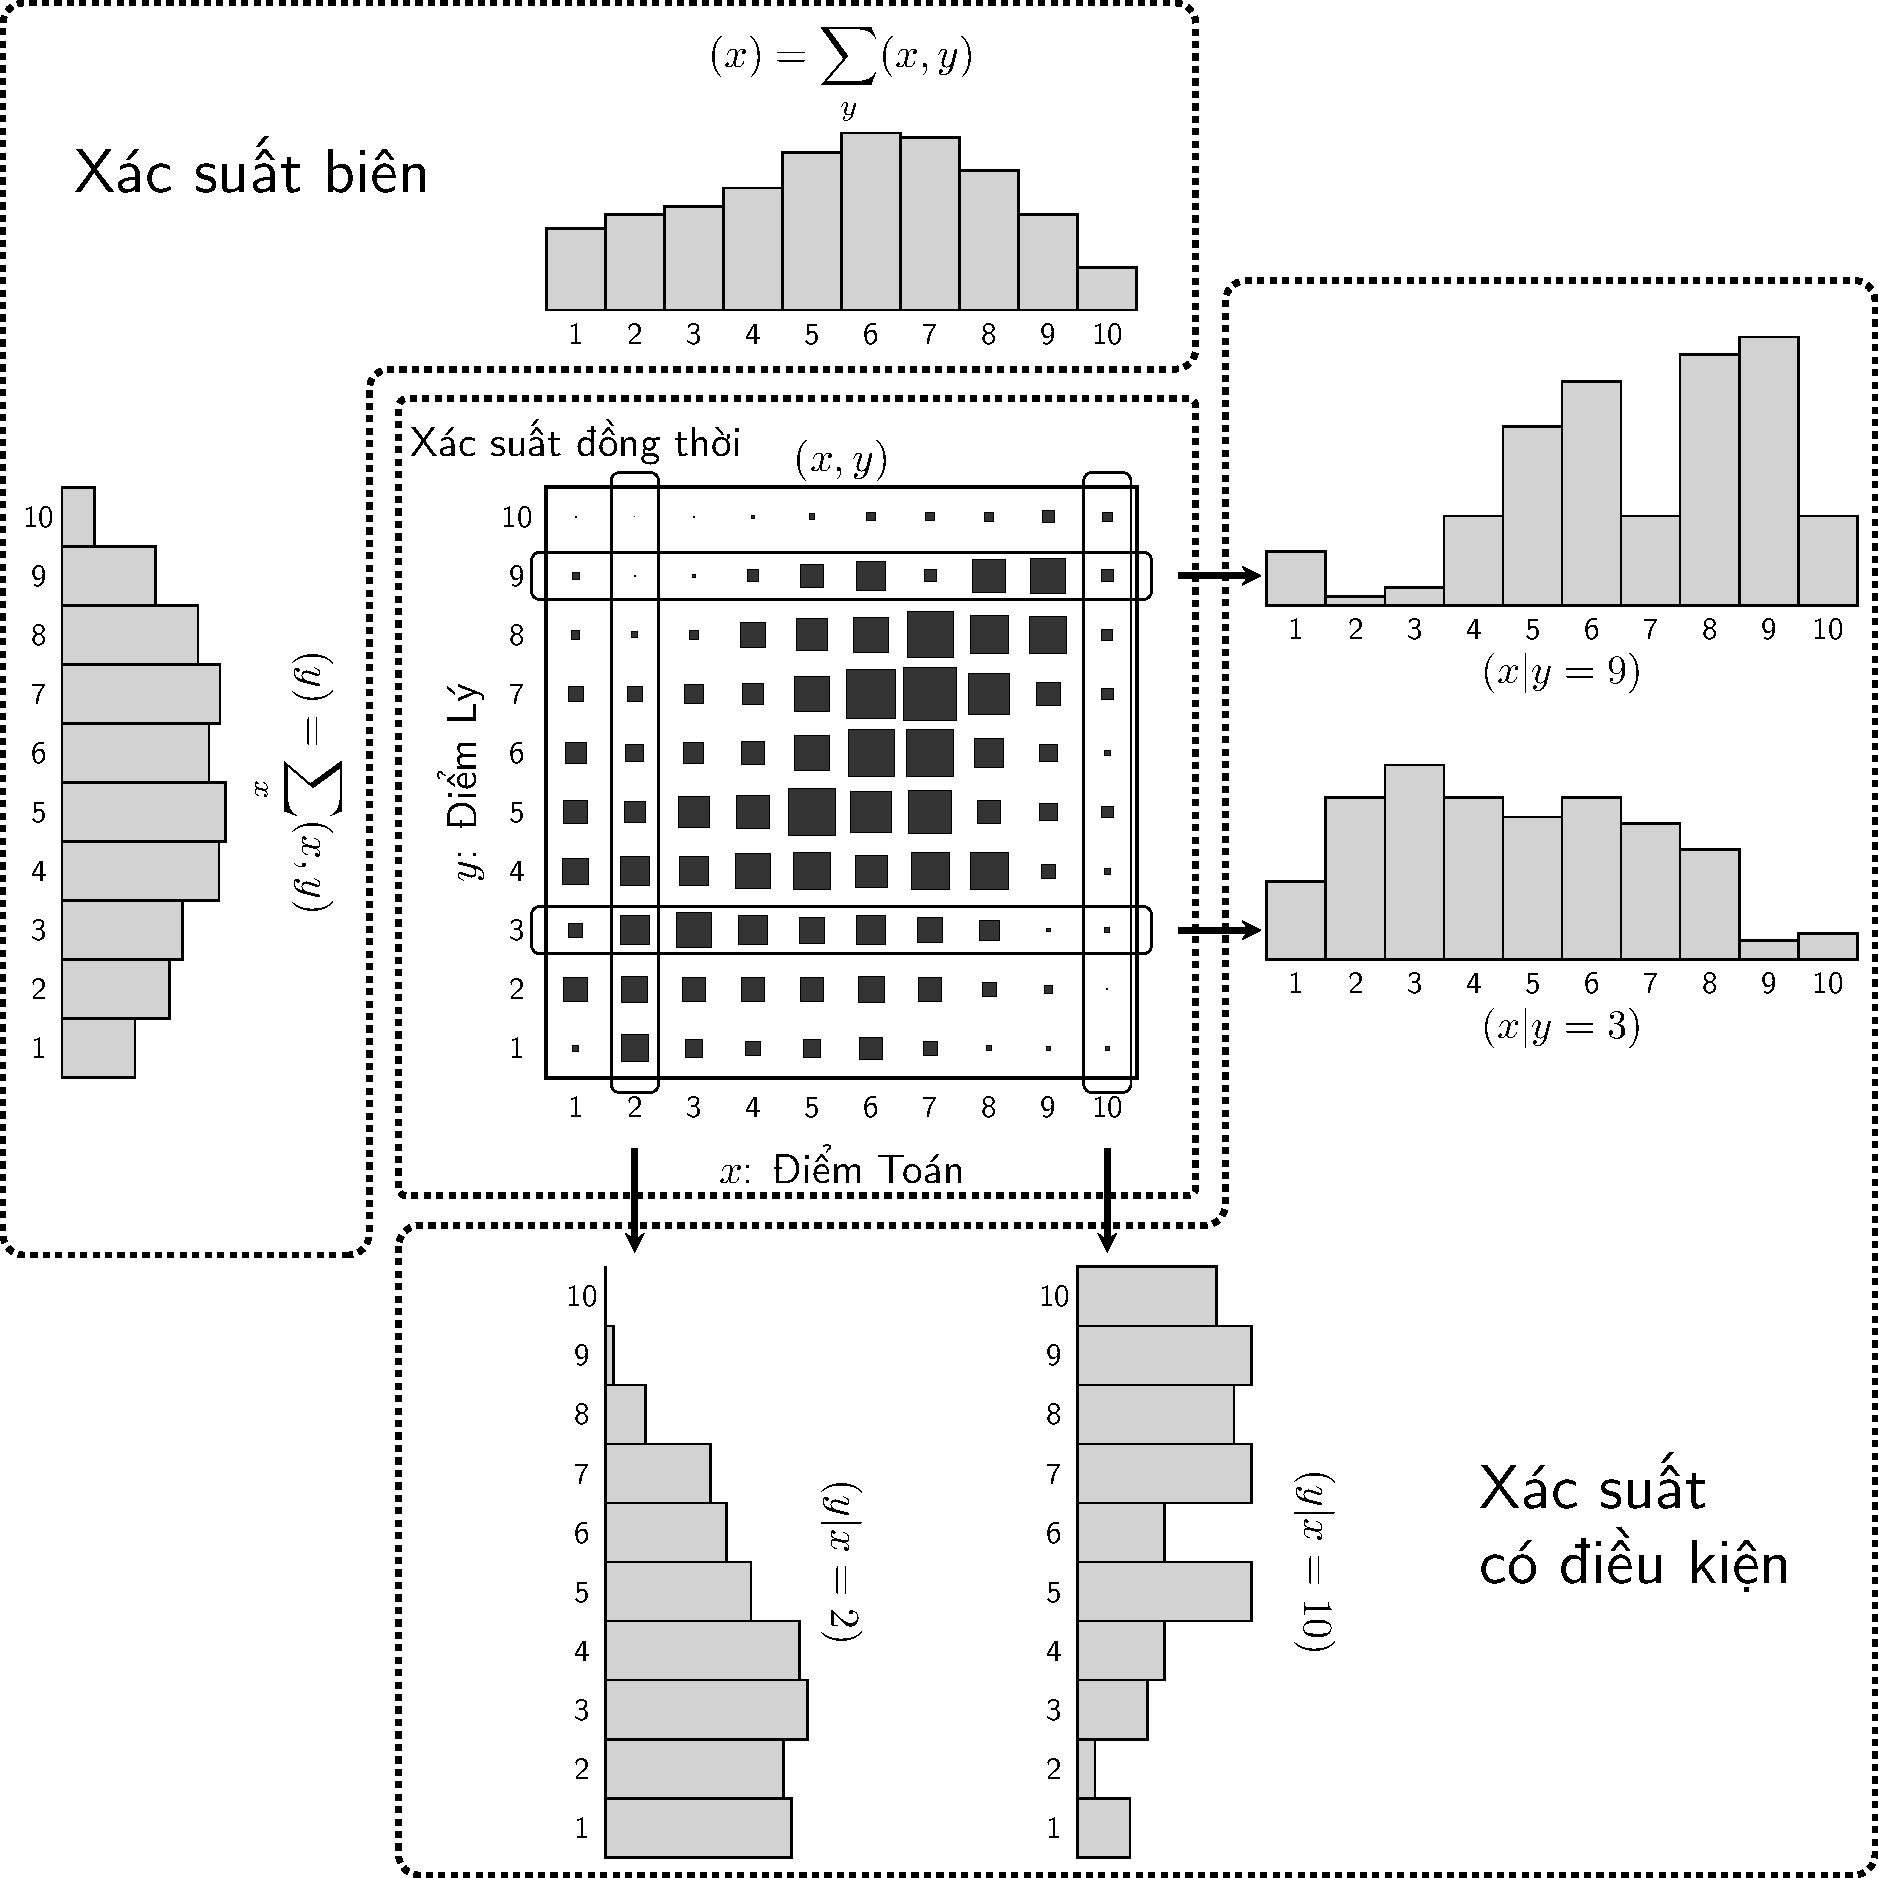
\includegraphics[width = \textwidth]{Chapters/02_LinearAlgebra/30_prob/latex/joint.pdf}
\caption[]{Xác suất đồng thời, xác suất biên, xác suất có điền kiện và mối quan hệ giữa chúng}
\label{fig:30_1}
\end{figure}

Thông thường, chúng ta sẽ làm việc với các bài toán ở đó xác suất được xác định
trên nhiều hơn hai biến ngẫu nhiên. Chẳng hạn, $p(x, y, z)$ thể hiện xác suất
đồng thời của ba biến ngẫu nhiên $x,y$ và $z$. Khi có nhiều biến ngẫu nhiên, ta
có thể viết chúng dưới dạng vector. Cụ thể, ta có thể viết $p(\mathbf{x})$ để
thể hiện xác suất của biến ngẫu nhiên nhiều chiều $\mathbf{x} =
[x_1, x_2, \dots, x_n]^T$. Khi có nhiều tập các biến ngẫu nhiên, ví dụ
$\mathbf{x}$ và $\mathbf{y}$, ta có thể viết $p(\mathbf{x},
\mathbf{y})$ để thể hiện xác suất đồng thời của tất cả các thành phần trong
hai biến ngẫu nhiên nhiều chiều này.

\subsection{Xác suất biên}
\index{xác suất biên -- marginalization}
\index{marginalization -- xác suất biên}
Nếu biết xác suất đồng thời của nhiều biến ngẫu nhiên, ta cũng có thể xác định
được phân phối xác suất của từng biến bằng cách lấy tổng (với biến ngẫu nhiên rời
rạc) hoặc tích phân (với biến ngẫu nhiên liên tục) theo tất cả các biến còn lại:% \begin{equation}
\begin{align}
\label{eqn:30_3}
\text{Nếu} ~x, y ~\text{rời rạc:}~ &p(x) = \sum_{y}p(x, y), \\
\label{eqn:30_4}
&p(y) = \sum_{x}p(x, y). \\
\label{eqn:30_5}
\text{Nếu} ~x, y ~\text{liên tục:}~ &p(x) = \int p(x, y)dy, \\
\label{eqn:30_6}
&p(y) = \int p(x, y)dx.
\end{align}
% \end{equation}
Với nhiều biến hơn, chẳng hạn bốn biến rời rạc $x, y, z, w$, cách tính được thực
hiện tương tự:
\index{xác suất biên -- marginal probability}
\index{marginal probability -- xác suất biên}
% \begin{equaton}
\begin{align}
\label{eqn:30_7}
p(x) &= \sum \limits_{ y, z, w}p(x, y, z, w),\\
\label{eqn:30_8}
p(x, y) &= \sum \limits_{z, w}p(x, y, z, w).
\end{align}
Cách xác định xác suất của một biến dựa trên xác suất đồng thời của nó với các
biến khác được gọi là \textit{phép biên hoá} (marginalization). Xác suất đó được gọi là
\textit{xác suất biên} (marginal probability).

\index{phép biên hóa -- marginalization}
\index{marginalization -- phép biên hóa}

Từ đây trở đi, nếu không đề cập gì thêm, chúng ta sẽ dùng ký hiệu $\sum$ để chỉ
chung cho cả hai loại biến ngẫu nhiên rời rạc và liên tục. Nếu biến là liên tục,
ta sẽ ngầm hiểu rằng dấu tổng ($\sum$) cần được thay bằng dấu tích phân
($\int$), biến lấy vi phân chính là biến được viết dưới dấu $\sum$. Chẳng hạn,
trong~\eqref{eqn:30_8}, nếu $z$ là liên tục, $w$ là rời rạc, công thức đúng sẽ
là
\begin{equation}
p(x, y) = \sum_{w}\left( \int p(x, y, z, w)dz \right) = \int \left( \sum_{w} p(x, y, z, w)\right) dz.
\end{equation}
Quay lại ví dụ trong Hình~\ref{fig:30_1} với hai biến ngẫu nhiên rời rạc $x, y$.
Lúc này, $p(x)$ được hiểu là xác suất để một học sinh đạt được $x$ điểm môn
Toán. Xác suất này được biểu thị ở khu vực ``Xác suất biên''. Có hai cách tính
xác suất này. Cách thứ nhất là đếm số học sinh được $x$ điểm môn toán rồi chia
cho tổng số học sinh. Cách thứ hai dựa trên xác suất đồng thời để một học sinh
được $x$ điểm môn Toán và $y$ điểm môn Lý. Số lượng học sinh đạt $x = x^*$ điểm
môn Toán sẽ bằng tổng số học sinh đạt $x = x^*$ điểm môn Toán \textit{và} $y$
điểm môn Lý, với $y$ là một giá trị bất kỳ từ 1 đến 10. vì vậy, để tính xác suất
$p(x)$, ta chỉ cần tính tổng của toàn bộ $p(x, y)$ với $y$ chạy từ 1 đến 10.

Dựa trên nhận xét này, mỗi giá trị của $p(x)$ chính bằng tổng các giá trị trong
cột thứ $x$ của hình vuông trung tâm. Mỗi giá trị của $p(y)$ sẽ bằng tổng các
giá trị trong hàng thứ $y$ tính từ đưới lên của hình vuông đó. Chú ý rằng tổng
các xác suất luôn bằng một.


\subsection{Xác suất có điều kiện.}
\index{xác suất có điều kiện -- conditional probability}
\index{conditional probability -- xác suất có điều kiện}

{Dựa vào phân phối điểm của các học sinh, liệu ta có thể tính được xác suất để
một học sinh được điểm 10 môn Lý, biết rằng học sinh đó được điểm 1 môn Toán?}

Xác suất để một biến ngẫu nhiên $x$ nhận một giá trị nào đó biết
rằng biến ngẫu nhiên $y$ có giá trị $y^*$ được gọi là \textit{xác suất có điều
kiện} (conditional probability), ký hiệu là $p(x| y = y^*)$.
% (đọc là \textit{probability of $x$ given that $y$ takes value $y^*$}).


Xác suất có điều kiện $p(x | y = y^*)$ có thể được tính dựa trên xác suất đồng
thời $p(x, y)$. Quay lại Hình~\ref{fig:30_1} ở khu vực ``Xác suất có điều
kiện''. Nếu biết rằng $y = 9$, xác suất $p(x | y = 9)$ có thể tính được dựa trên
hàng thứ chín của hình vuông trung tâm, tức hàng $p(x, y = 9)$. Xác suất $p(x | y =
9) $ lớn nếu $p(x, y= 9)$ lớn. Chú ý rằng tổng các xác suất $\sum_{x} p(x,
y = 9)$ nhỏ hơn một, và bằng tổng các xác suất trên hàng thứ chín này. Để thoả
mãn điều kiện tổng các xác suất bằng một, ta cần chia mỗi đại lượng $p(x, y =
9)$ cho tổng của hàng này, tức là
\begin{equation}
p(x | y = 9) =\frac{p(x, y = 9)}{\sum \limits_x p(x, y = 9)} =
\frac{p(x, y = 9)}{p(y = 9)}.
\end{equation}
Tổng quát,
\begin{equation}
\label{eqn:30_9}
\displaystyle
p(x|y = y^*) = \frac{p(x, y = y^*)}{\sum \limits_{x} p(x, y = y^*)} =
\frac{p(x, y = y^*)}{p(y = y^*)},
\end{equation}
ở đây ta đã sử dụng công thức tính xác suất biên trong~\eqref{eqn:30_4} cho mẫu
số. Thông thường, ta có thể viết xác suất có điều kiện mà không cần chỉ rõ giá trị $y = y^*$ và có các công thức gọn hơn:
\begin{equation}
\label{eqn:30_2}
p(x |y) = \frac{p(x, y)}{p(y)}, ~p(y | x) = \frac{p(y, x)}{p(x)}.
\end{equation}

Từ đó ta có quan hệ
\begin{equation}
\label{eqn:30_11}
p(x, y) = p(x|y)p(y) = p(y | x) p(x).
\end{equation}
Khi có nhiều hơn hai biến ngẫu nhiên, ta có các công thức
\begin{eqnarray}
\label{eqn:30_12}
p(x, y, z, w)
& = & p(x, y, z | w) p(w) \\
\label{eqn:30_13}
& = & p(x, y | z, w)p(z, w) = p(x, y | z, w) p(z | w) p(w) \\
\label{eqn:30_14}
& = & p(x | y, z, w)p(y | z, w) p(z | w) p(w).
\end{eqnarray}

Công thức \eqref{eqn:30_14} có dạng {chuỗi} và được sử dụng nhiều sau
này.


\subsection{Quy tắc Bayes}
\index{quy tắc Bayes -- Bayes' rule}
\index{Bayes' rule -- quy tắc Bayes}
Công thức \eqref{eqn:30_11} biểu diễn xác suất đồng thời theo hai cách. Từ đó có thể suy ra
\begin{equation}
p(y |x) p(x) = p(x | y) p(y).
\end{equation}
Biến đối một chút:
% \begin{equation}
% \displaystyle
\begin{align}
\label{eqn:30_15}
p(y | x)
& =  \frac{p(x |y) p(y)}{p(x)} \\
\label{eqn:30_16}
& =  \frac{p(x |y) p(y)}{\sum \limits_{y} p(x, y)} \\
\label{eqn:30_17}
& =  \frac{p(x |y) p(y)}{\sum \limits_{y} p(x | y) p(y)}.
\end{align}
% \end{equation}
Trong dòng thứ hai và thứ ba, các công thức về xác suất biên và xác suất đồng thời
ở mẫu số đã được sử dụng. Từ~\eqref{eqn:30_17} ta có thể thấy rằng $p(y | x)$
hoàn toàn có thể tính được nếu ta biết mọi $p(x | y)$ và $p(y)$. Tuy nhiên, việc
tính trực tiếp xác suất này thường phức tạp.

% Thay vào đó, ta có thể đi tìm mô
% hình phù hợp của $p(\mathbf{x} | y)$ trên training data sao cho \textit{những gì
% đã thực sự xảy ra có xác suất cao nhất có thể} (Chỗ này có thể hơi khó hình
% dung, tôi sẽ nói cụ thể về việc này trong bài tiếp theo). Dựa trên training
% data, các tham số của mô hình này có thể tìm được qua một bài toán tối ưu.

{Ba công thức \eqref{eqn:30_15}-\eqref{eqn:30_17} thường được gọi là \textit{quy
tắc Bayes}. Chúng được sử dụng rộng rãi trong machine learning}

% Trong Machine Learning, chúng ta thường mô tả quan hệ giữa hai biến $x$ và $y$
% dưới dạng xác suất có điều kiện $p(y|x)$. Ví dụ, biết rằng đầu vào là một bức
% ảnh ở dạng vector $\mathbf{x}$, xác suất để bức ảnh chứa một chiếc xe là bao nhiêu. Khi đó, ta phải tính $p(y | \mathbf{x})$.

% \textbf{Ví dụ}: Tại một bệnh viện, giả sử chúng ta quan tâm tới việc xét nghiệm
% một bệnh nhân có
% bệnh ung thư phổi hay không nếu anh/cô ấy hút thuốc. Biết rằng xác xuất một
% bệnh nhân vào xét nghiệm trong bệnh viện đó có bệnh ung thư phổi là 0.1.


\subsection{Biến ngẫu nhiên độc lập}
\index{biến ngẫu nhiên độc lập -- independent random variables}
\index{independent random variables -- biến ngẫu nhiên độc lập}
Nếu biết giá trị của một biến ngẫu nhiên $x$ không mang lại thông tin về việc
suy ra giá trị của biến ngẫu nhiên $y$ và ngược lại, thì ta nói rằng hai biến
ngẫu nhiên này là \textit{độc lập}. Chẳng hạn, chiều cao của một học sinh và
điểm thi môn Toán của học sinh đó có thể coi là hai biến ngẫu nhiên {độc lập}.
Khi hai biến ngẫu nhiên $x$ và $y$ là {độc lập}, ta  có% \begin{equation}
\begin{eqnarray}
\label{eqn:30_18}
p(x | y) &=& p(x),  \\
\label{eqn:30_19}
p(y | x) &=& p(y).
\end{eqnarray}
% \end{equation}
Thay vào biểu thức xác suất đồng thời trong \eqref{eqn:30_11}, ta có
\begin{equation}
\label{eqn:30_20}
p(x, y) = p(x | y) p(y) = p(x) p(y).
\end{equation}


\subsection{Kỳ vọng}
\label{sub:expectaion_covariance}
\index{kỳ vọng -- expectation}
\index{expectation -- kỳ vọng}
\textit{Kỳ vọng} (expectation) của một biến ngẫu nhiên $x$ được định nghĩa bởi% \begin{equation}
\begin{eqnarray}
\label{eqn:30_21}
\text{E}[x] = \sum_x x p(x)  & \text{nếu}~ x ~ \text{là rời rạc.} \quad
\\
\label{eqn:30_22}
\text{E}[x] = \int x p(x) dx  & \text{nếu}~ x ~ \text{là liên tục.}
\end{eqnarray}
% \end{equation}
Giả sử $f(.)$ là một hàm số trả về một số với mỗi giá trị $x^*$ của biến ngẫu
nhiên $x$. Khi đó, nếu $x$ là biến ngẫu nhiên rời rạc, ta có
\begin{equation}
\label{eqn:30_23}
\text{E}[f(x)] = \sum_x f(x) p(x).
\end{equation}
Công thức cho biến ngẫu nhiên liên tục cũng được viết tương tự.

Với xác suất đồng thời, kỳ vọng của một hàm cũng được xác định tương tự:
\begin{equation}
\label{eqn:30_24}
\text{E}[f(x, y)] = \sum_{x,y} f(x, y) p(x, y) dx dy.
\end{equation}
Có ba tính chất cần nhớ về kỳ vọng:
\begin{enumerate}
\item Kỳ vọng của một hằng số theo một biến ngẫu nhiên $x$ bất kỳ bằng chính hằng số đó:
\begin{equation}
\label{eqn:30_25}
\text{E}[\alpha] = \alpha.
\end{equation}
\item Kỳ vọng có tính chất tuyến tính:
\begin{eqnarray}
\label{eqn:30_26}
\text{E}[\alpha x] & = & \alpha \text{E}[x],  \\
\label{eqn:30_27}
\text{E}[f(x) + g(x)] & = & \text{E}[f(x)] + \text{E}[g(x)].
\end{eqnarray}
\item Kỳ vọng của tích hai biến ngẫu nhiên độc lập bằng tích kỳ vọng của chúng:
\begin{equation}
\label{eqn:30_28}
\text{E}[f(x) g(y)] = \text{E}[f(x)] \text{E}[g(y)].
\end{equation}

\end{enumerate}


% \subsection{Kỳ vọng và ma trận hiệp phương sai}

Khái niệm kỳ vọng thường đi kèm với khái niệm \textit{phương
sai} (variance) trong không gian một chiều và \textit{ma trận hiệp
phương sai} (covariance matrix) trong không gian nhiều chiều.

\subsection{Phương sai} % (fold)

% \subsubsection{Với dữ liệu một chiều}
\index{phương sai -- variance}
\index{variance -- phương sai}
\index{do@độ lệch chuẩn -- standard deviation}
\index{standard deviation -- độ lệch chuẩn}
Cho $N$ giá trị $x_1, x_2, \dots, x_N$. {Kỳ vọng} và {phương sai}
của bộ dữ liệu này được tính theo công thức
\begin{eqnarray}
\bar{x} &=& \frac{1}{N}\sum_{n=1}^N x_n = \frac{1}{N}\mathbf{x1},\\\
\sigma^2 &=& \frac{1}{N} \sum_{n=1}^N (x_n - \bar{x})^2,
\end{eqnarray}
với $\bx = \bmt x_1, x_2, \dots, x_N\emt $, và $\mathbf{1} \in \mathbb{R}^N$ là
vector cột chứa toàn phần tử 1. Kỳ vọng đơn giản là trung bình cộng của toàn bộ
các giá trị. Phương sai là trung bình cộng của bình phương khoảng cách từ mỗi
điểm tới kỳ vọng. Phương sai càng nhỏ, các điểm dữ liệu càng gần với kỳ vọng,
tức các điểm dữ liệu càng giống nhau. Phương sai càng lớn, dữ liệu càng có tính
phân tán. Ví dụ về kỳ vọng và phương sai của dữ liệu một chiều có thể được thấy
trong Hình~\ref{fig:27_2a}.

Căn bậc hai của phương sai, $\sigma$ còn được gọi là \textit{độ lệch chuẩn} (standard deviation) của
dữ liệu.


%%%%%%% Three subfigures with bottom caption%%%%%%%%%%%%%%
\begin{figure}[t]
\begin{subfigure}{0.325\textwidth}
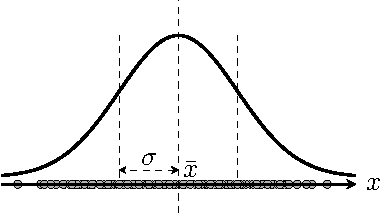
\includegraphics[width=0.99\linewidth]{Chapters/07_DimemsionalityReduction/27_pca/latex/var_1d.pdf}
\caption{}
\label{fig:27_2a}
\end{subfigure}
\begin{subfigure}{0.325\textwidth}
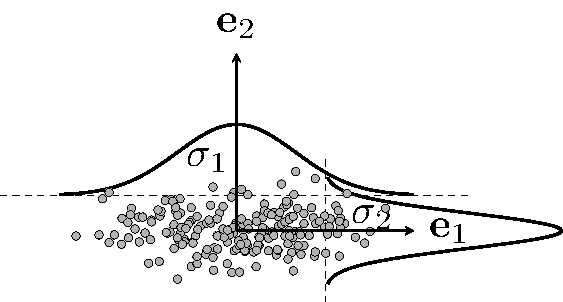
\includegraphics[width=0.99\linewidth]{Chapters/07_DimemsionalityReduction/27_pca/latex/pca_diagvar.pdf}
\caption{}
\label{fig:27_2b}
\end{subfigure}
\begin{subfigure}{0.325\textwidth}
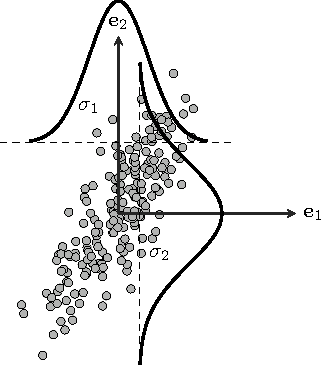
\includegraphics[width=0.99\linewidth]{Chapters/07_DimemsionalityReduction/27_pca/latex/pca_var0.pdf}
\caption{}
\label{fig:27_2c}
\end{subfigure}
\caption{
Ví dụ về kỳ vọng và phương sai. (a) Dữ liệu trong không gian
một chiều. (b) Dữ liệu trong không gian hai chiều mà hai chiều
không tương quan. Trong trường hợp này, ma trận hiệp phương sai là ma trận
đường chéo với hai phần tử trên đường chéo  là $\sigma_1, \sigma_2$, đây
cũng chính là hai trị riêng của ma trận hiệp phương sai và là phương sai
của mỗi chiều dữ liệu. (c) Dữ liệu trong không gian hai chiều có tương
quan. Theo mỗi chiều, ta có thể tính được kỳ vọng và phương sai. Phương sai
càng lớn thì dữ liệu trong chiều đó càng phân tán. Trong ví dụ này, dữ liệu
theo chiều thứ hai phân tán nhiều hơn so với chiều thứ nhất. }
\label{fig:27_2}
\end{figure}

\subsection{Ma trận hiệp phương sai}

Cho $N$ điểm dữ liệu được biểu diễn bởi các vector cột $\mathbf{x}_1, \dots, \mathbf{x}_N$, khi đó, {vector kỳ vọng} và {ma trận hiệp phương sai} của toàn bộ dữ liệu được định nghĩa là
\begin{eqnarray}
\bar{\mathbf{x}} &=& \frac{1}{N} \sum_{n=1}^N \mathbf{x}_n, \\\
\mathbf{S} &=&  \frac{1}{N}\sum_{n=1}^N (\mathbf{x}_n - \bar{\mathbf{x}})(\mathbf{x}_n - \bar{\mathbf{x}})^T = \frac{1}{N}\hat{\mathbf{X}}\hat{\mathbf{X}}^T.
\end{eqnarray}
Trong đó $\hat{\mathbf{X}}$ được tạo bằng cách trừ mỗi cột của $\mathbf{X}$ đi $\bar{\mathbf{x}}$:
\begin{equation}
\hat{\mathbf{x}}_n = \mathbf{x}_n - \bar{\mathbf{x}}.
\end{equation}
\newpage
Một vài tính chất của ma trận hiệp phương sai:
\begin{enumerate}

\item Ma trận hiệp phương sai là một ma trận đối xứng, hơn nữa, nó là một ma trận \href{https://machinelearningcoban.com/2017/03/12/convexity/#positive-semidefinite}{nửa xác định dương}.

\item Mọi phần tử trên đường chéo của ma trận hiệp phương sai là các số không âm. Chúng chính là phương sai của từng chiều dữ liệu.

\item Các phần tử ngoài đường chéo $s_{ij}, i \neq j$ thể hiện sự tương quan
giữa thành phần thứ $i$ và thứ $j$ của dữ liệu, còn được gọi là hiệp phương
sai. Giá trị này có thể dương, âm hoặc bằng không. Khi nó bằng không, ta nói
rằng hai thành phần $i, j$ trong dữ liệu là \textit{không tương quan}.

\item Nếu ma trận hiệp phương sai là ma trận đường chéo, ta có dữ liệu hoàn toàn không tương quan giữa các chiều.
\end{enumerate}

Ví dụ về sự tương quan của dữ liệu được cho trong Hình~\ref{fig:27_2b} và
\ref{fig:27_2c}.% <hr>
% <div>
% <table width = "100%" style = "border: 0px solid white">
%     <tr >
%         <td width="40%" style = "border: 0px solid white" align = "center">
%         <img style="display:block;" width = "100%" src = "/assets/27_pca/var_1d.png">
%          <br>
%         a)
%          </td>
%          <td width="40%" style = "border: 0px solid white" align = "center">
%          <img style="display:block;" width = "100%" src = "/assets/27_pca/pca_diagvar.png">
%           <br>
%          b)
%           </td>
%     </tr>

%     <tr >
%         <td width="40%" style = "border: 0px solid white" align = "center">
%         <img style="display:block;" width = "100%" src = "/assets/27_pca/pca_var0.png">
%          <br>
%         c)
%          </td>
%          <td width="40%" style = "border: 0px solid white" align = "justify">
%         Hình 2: Ví dụ về kỳ vọng và phương sai. a) Trong không gian 1 chiều. b) Không gian 2 chiều mà hai chiều không tương quan. Trong trường hợp này, ma trận hiệp phương sai là ma trận đường chéo với hai phần tử trên đường chéo  là $\sigma_1, \sigma_2$, đây cũng chính là hai trị riêng của ma trận hiệp phương sai và là phương sai của mỗi chiều dữ liệu. c) Dữ liệu trong không gian hai chiều có tương quan. Theo mỗi chiều, ta có thể tính được kỳ vọng và phương sai. Phương sai càng lớn thì dữ liệu trong chiều đó càng phân tán. Trong ví dụ này, dữ liệu theo chiều thứ hai phân tán nhiều hơn so so với chiều thứ nhất.
%           </td>
%     </tr>
% </table>
% </div>
% <hr>


\section{Một vài phân phối thường gặp}
\index{phân phối xác suất -- probability distribution}
\index{probability distribution -- phân phối xác suất}
\subsection{Phân phối Bernoulli}
\index{phân phối xác suất -- probability distribution!phân phói Bernoulli}
\index{probability distribution -- phân phối xác suất!phân phói Bernoulli}

Phân phối Bernoulli là một phân phối rời rạc mô tả các biến ngẫu nhiên nhị
phân với đầu ra chỉ nhận một trong hai giá trị $x \in \{0, 1\}$. Hai giá trị
này có thể là \textit{xấp} và \textit{ngửa} khi tung đồng xu; có thể là
\textit{giao dịch lừa đảo} và \textit{giao dịch thông thường} trong bài toán
xác
định giao dịch lừa đảo trong tín dụng; có thể là \textit{người} và \textit{không
phải người} trong bài toán xác định xem trong một bức ảnh có người hay không.

Phân phối Bernoulli được mô tả bằng một tham số $\lambda \in [0, 1]$. Xác suất của mỗi đầu ra là
\begin{equation}
\label{eqn:30_29}
p(x = 1) = \lambda, ~~~~ p(x = 0) = 1 - p(x = 1) = 1 - \lambda.
\end{equation}
Hai đẳng thức này thường được viết gọn lại thành
\begin{equation}
\label{eqn:30_292}
p(x) = \lambda^x (1 - \lambda)^{1 - x},
\end{equation}
với giả định $0 ^0 = 1$. Thật vậy, $p(0) = \lambda^0 (1 - \lambda)^1 = 1 -
\lambda$, và $p(1) = \lambda^1 (1 - \lambda)^0 = \lambda$.


Phân phối Bernoulli thường được ký hiệu ngắn gọn dưới dạng
\begin{equation}
\label{eqn:30_30}
p(x) = \text{Bern}_x [\lambda].
\end{equation}

\subsection{Phân phối categorical}
\index{phân phối xác suất -- probability distribution!phân phối categorical}
\index{probability distribution -- phân phối xác suất!phân phối categorical}
Trong nhiều trường hợp, đầu ra của biến ngẫu nhiên rời rạc có thể nhận nhiều hơn
hai giá trị. Ví dụ, một bức ảnh có thể chứa một chiếc xe, một người, hoặc một
con mèo. Khi đó, ta dùng một phân phối tổng quát của phân phối Bernoulli, được
gọi là \textit{phân phối categorical}. Các đầu ra được mô tả bởi một phần tử
trong tập hợp $\{1, 2, \dots, K\}$.

Nếu có $K$ đầu ra, phân phối categorical sẽ được mô tả bởi $K$ tham số, viết
dưới dạng vector $\lambda = [\lambda_1, \lambda_2, \dots, \lambda_K]$ với các
$\lambda_k$ không âm và có tổng bằng một. Mỗi giá trị $\lambda_k$ thể hiện xác
suất để đầu ra nhận giá trị $k$:
\begin{math}
p(x = k) = \lambda_k
\end{math}.
\index{biểu diễn one-hot -- one-hot encoding}
\index{one-hot encoding -- biểu diễn one-hot}

Phân phối categorical thường được ký hiệu dưới dạng:
\begin{equation}
p(x) = \text{Cat}_x [\lambda].
\end{equation}
Cách biểu diễn đầu ra là một số $k$ trong tập hợp $\{1, 2, \dots, K\}$ có thể
được thay bằng biểu diễn \textit{one-hot}. Mỗi vector one-hot là một vector $K$
phần tử, trong đó $K-1$ phần tử bằng 0, một phần tử bằng 1 tại vị trí ứng với
đầu ra $k$. Nói cách khác, mỗi đầu ra là một trong các vector đơn vị bậc $K$:
$\{\mathbf{e}_1, \mathbf{e}_2,\dots, \mathbf{e}_K\}$. Ta có thể viết
\begin{equation}
\label{eqn:30_31}
p(x = k) = p(\mathbf{x} = \mathbf{e}_k) = \prod_{j=1}^K \lambda_j^{x_j} = \lambda_k.
\end{equation}
Dấu bằng cuối cùng xảy ra vì $x_k = 1, x_j = 0~\forall j \neq k$.
% Cách viết này được sử dụng rất nhiều trong Machine Learning.
% Thay vào~\eqref{eqn:30_31} ta sẽ được $p(\bx = \be_k) = \lambda_k = p(x = k)$.


\subsection{Phân phối chuẩn một chiều}
\index{phân phối xác suất -- probability distribution!phân phối chuẩn một chiều -- univariate normal distribution}
\index{probability distribution -- phân phối xác suất!univariate normal distribution -- phân phối chuẩn một chiều}

\textit{Phân phối chuẩn một chiều} (univariate normal distribution) được định nghĩa trên các biến liên tục nhận giá
trị $x \in (-\infty, \infty)$. Đây là một phân phối được sử dụng nhiều nhất với
các biến ngẫu nhiên liên tục. Phân phối này được mô tả bởi hai tham số:
{kỳ vọng} $\mu$ và {phương sai} $\sigma^2$.

Hàm mật độ xác suất của phân phối này được định nghĩa bởi
\begin{equation}
\label{eqn:30_32}
p(x) = \frac{1}{\sqrt{2\pi \sigma^2}}\exp \left( -\frac{(x - \mu)^2}{2\sigma^2}\right).
\end{equation}
Hàm mật độ này thường được viết gọn dưới dạng $p(x) = \text{Norm}_x [\mu,
\sigma^2]$ hoặc $\mathcal{N}(\mu, \sigma^2)$.

Ví dụ về đồ thị hàm mật độ xác suất của phân phối chuẩn một chiều được biểu thị
trên Hình~\ref{fig:30_2a}.

\begin{figure}[t]
\begin{subfigure}{0.49\textwidth}
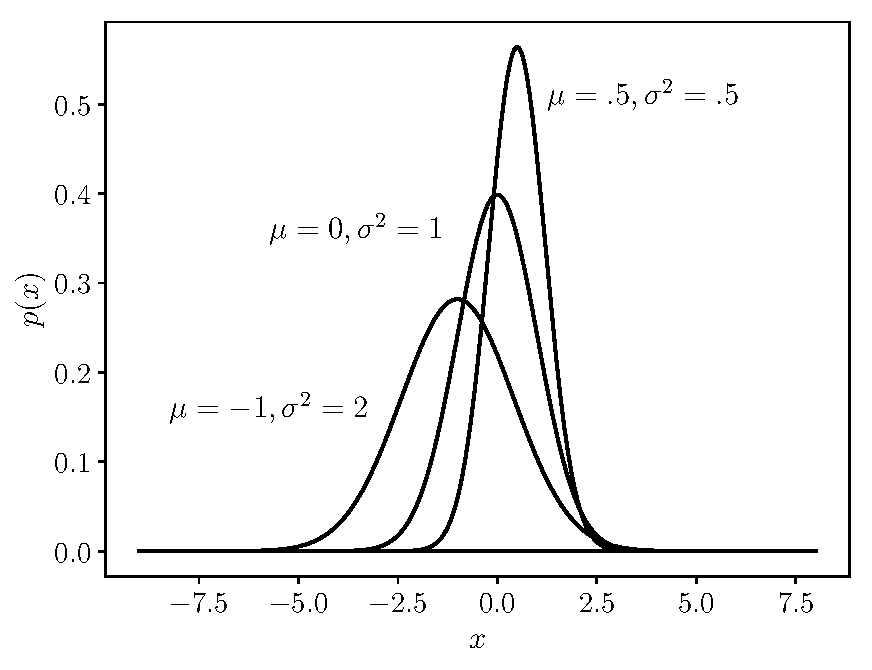
\includegraphics[width=0.99\linewidth]{Chapters/02_LinearAlgebra/30_prob/python/uni_norm.pdf}
\caption{}
\label{fig:30_2a}
\end{subfigure}
\begin{subfigure}{0.49\textwidth}
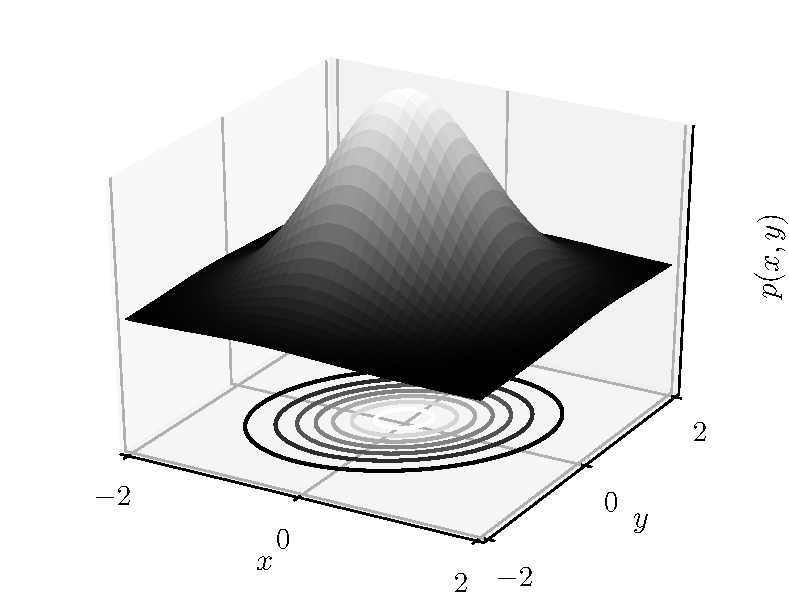
\includegraphics[width=0.99\linewidth]{Chapters/02_LinearAlgebra/30_prob/python/bi_norm.pdf}
% 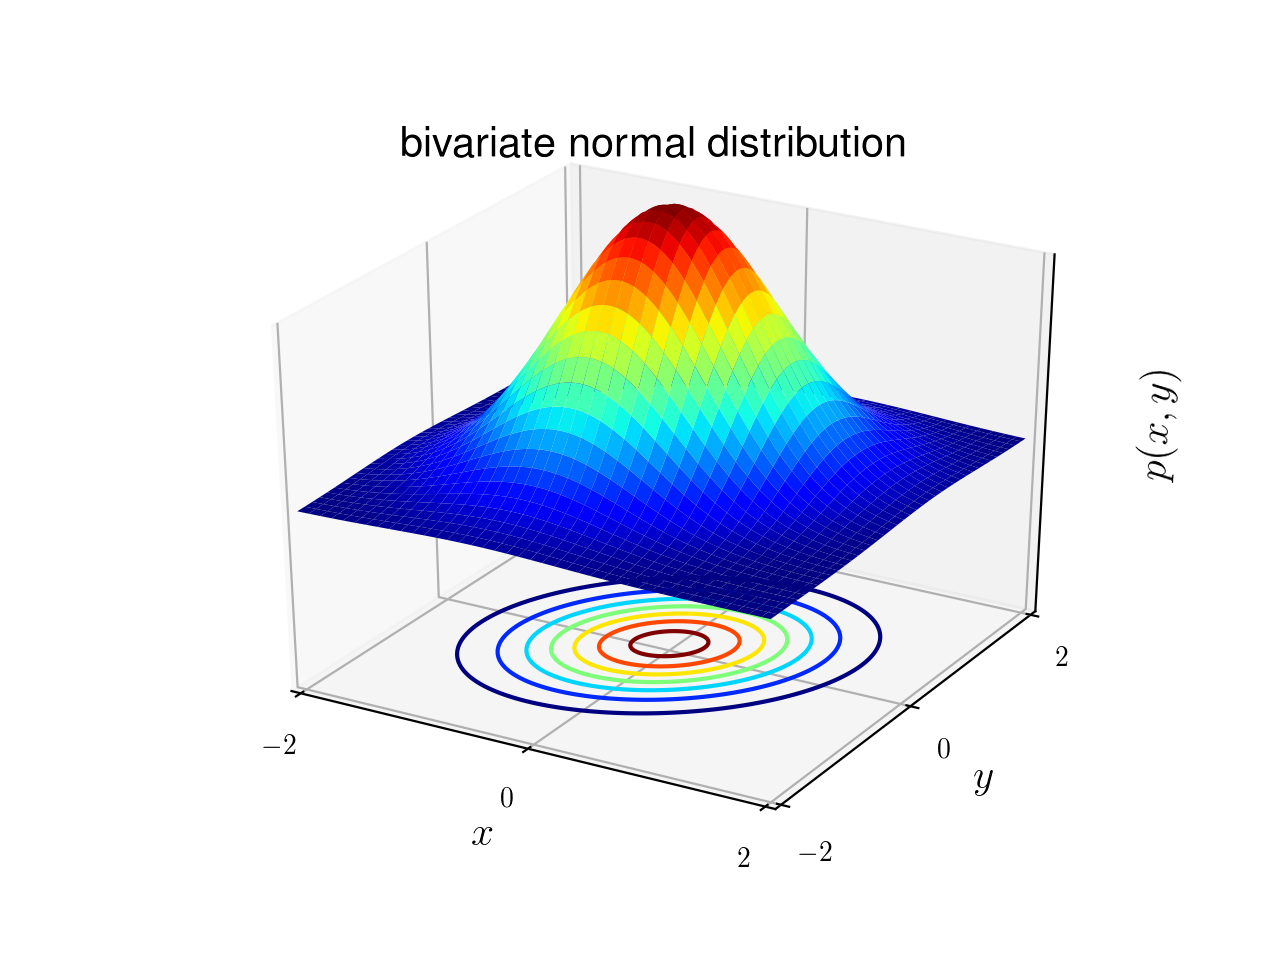
\includegraphics[width=0.99\linewidth]{Chapters/02_LinearAlgebra/30_prob/bivariate.png}
\caption{}
\label{fig:30_2b}
\end{subfigure}
\caption{
Ví dụ về hàm mật độ xác suất của (a) phân phối chuẩn một chiều, và (b) phân
phối chuẩn hai chiều.}
\label{fig:30_2}
\end{figure}

\subsection{Phân phối chuẩn nhiều chiều}
\index{phân phối xác suất -- probability distribution!phân phối chuẩn nhiều chiều -- multivariate normal distribution}
\index{probability distribution -- phân phối xác suất!multivariate normal distribution -- phân phối chuẩn nhiều chiều}

\textit{Phân phối chuẩn nhiều chiều} (multivariate normal distribution) là trường hợp tổng quát của phân phối chuẩn khi biến
ngẫu nhiên là nhiều chiều, giả sử là $D$ chiều. Có hai tham số mô tả phân phối
này là {vector kỳ vọng} $\bmu \in \mathbb{R}^D$ và {ma trận hiệp phương sai}
$\bSigma \in \mathbb{S}^D$ là một ma trận {đối xứng xác định dương}.

\newpage
Hàm mật độ xác suất có dạng
\begin{equation}
\label{eqn:30_33}
p(\mathbf{x}) = \frac{1}{(2\pi)^{D/2} |\bSigma|^{1/2}} \exp \left(-\frac{1}{2}
(\mathbf{x} - \bmu)^T \bSigma^{-1} (\mathbf{x} - \bmu)\right),
\end{equation}
với $|\bSigma|$ là định thức của ma trận hiệp phương sai $\bSigma$.

Hàm mật độ này thường được viết gọn lại dưới dạng
$p(\mathbf{x}) = \text{Norm}_{\mathbf{x}}[\bmu, \bSigma]$ hoặc
$\mathcal{N}(\bmu, \bSigma)$.

Ví dụ về hàm mật độ xác suất của một phân phối chuẩn hai chiều được mô tả bởi
một mặt cong trên Hình~\ref{fig:30_2b}. Nếu cắt mặt này theo các mặt phẳng
song song với mặt đáy, ta sẽ thu được các hình ellipse đồng tâm.

\subsection{Phân phối Beta}
\index{phân phối xác suất -- probability distribution!phân phối Beta}
\index{probability distribution -- phân phối xác suất!phân phối Beta}
Phân phối Beta là một phân phối liên tục được định nghĩa trên một biến ngẫu
nhiên $\lambda \in [0, 1]$. Phân phối Beta được dùng để mô tả {tham số} cho một
phân phối khác. Cụ thể, phân phối này phù hợp với việc mô tả sự {biến động} của
tham số $\lambda$ trong phân phối Bernoulli.

Phân phối Beta được mô tả bởi hai tham số {dương} $\alpha, \beta$. Hàm
mật độ xác suất của nó được cho bởi
\begin{equation}
\label{eqn:30_34}
p(\lambda) = \frac{\Gamma(\alpha + \beta)}{\Gamma(\alpha) \Gamma(\beta)} \lambda^{\alpha - 1} ( 1 - \lambda) ^{\beta - 1},
\end{equation}
với $\Gamma(.)$ là hàm số gamma, được định nghĩa bởi
\begin{equation}
\Gamma(z) = \int_0^{\infty} t^{z-1}\exp(-t) dt.
\end{equation}
% và có liên quan tới giai thừa khi $z$ là số tự nhiên:
% \begin{equation}
%   \Gamma[z] = (z-1)!
% \end{equation}

{Trên thực tế, việc tính giá trị của hàm số gamma không thực sự
quan trọng vì nó chỉ mang tính chuẩn hoá để tổng xác suất bằng một.}

Phân phối Beta thường được ký hiệu là $p(\lambda) =  \text{Beta}_{\lambda}[\alpha, \beta]$.

Hình~\ref{fig:30_3} minh hoạ hàm mật độ xác suất của phân phối Beta với các
cặp giá trị $(\alpha, \beta)$ khác nhau.

% ******************************************************************************
\begin{figure}[t]
\begin{subfigure}{0.325\textwidth}
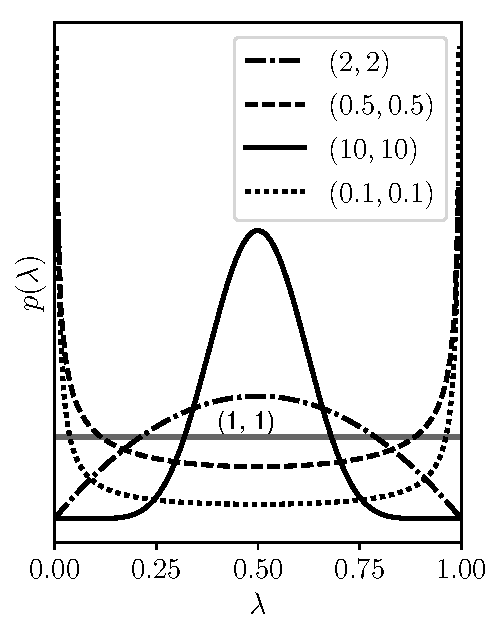
\includegraphics[width=0.99\linewidth]{Chapters/02_LinearAlgebra/30_prob/python/beta1.pdf}
\caption{$\alpha = \beta$}
\label{fig:30_3a}
\end{subfigure}
\begin{subfigure}{0.325\textwidth}
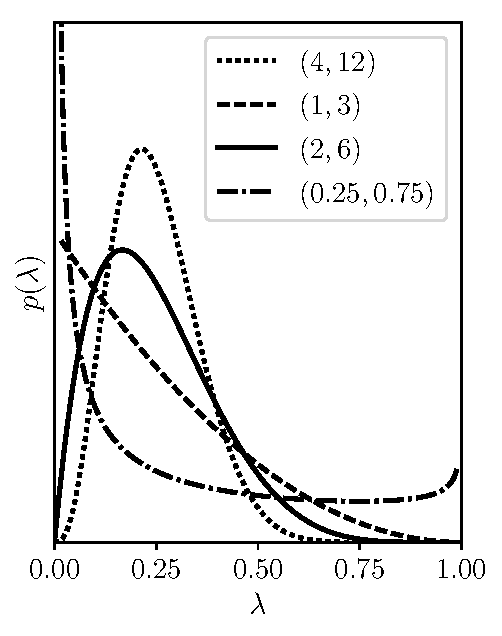
\includegraphics[width=0.99\linewidth]{Chapters/02_LinearAlgebra/30_prob/python/beta2.pdf}
\caption{$\alpha < \beta$}
\label{fig:30_3b}
\end{subfigure}
\begin{subfigure}{0.325\textwidth}
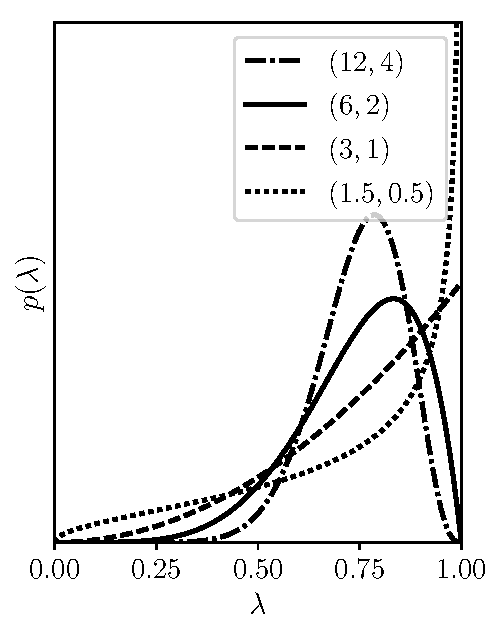
\includegraphics[width=0.99\linewidth]{Chapters/02_LinearAlgebra/30_prob/python/beta3.pdf}
\caption{$\alpha > \beta$}
\label{fig:30_3c}
\end{subfigure}
\caption{
Ví dụ về hàm mật độ xác suất của phân phối Beta. (a) $\alpha = \beta$, đồ thị
hàm số là đối xứng. (b) $\alpha < \beta$, đồ thị hàm số lệch sang trái, chứng tỏ xác suất $\lambda$ nhỏ là lớn. (c) $\alpha > \beta$, đồ thị hàm số lệch sang phải, chứng tỏ xác suất $\lambda$ lớn là lớn.
}
\label{fig:30_3}
\end{figure}
% ******************************************************************************

\begin{itemize}

\item Trong Hình \ref{fig:30_3a}, khi $\alpha =\beta$. Đồ thị của các hàm
mật độ xác suất đối xứng qua đường thẳng $\lambda = 0.5$. Khi $\alpha =
\beta = 1$, thay vào \eqref{eqn:30_34}, ta thấy $p(\lambda) = 1$ với mọi
$\lambda$. Trong trường hợp này, phân phối Beta trở thành \textit{phân phối
đều} Khi $\alpha = \beta > 1$, các hàm số đạt giá trị cao tại gần trung tâm,
tức $\lambda$ sẽ nhận giá trị xung quanh điểm 0.5 với xác suất cao. Khi
$\alpha = \beta < 1$, hàm số đạt giá trị cao tại các điểm gần 0 và 1.    % Điều này chứng tỏ Bernoulli distribution tương ứng với các $\lambda$ này
% bị thiên lệch nhiều.

\item Trong Hình~\ref{fig:30_3b}, khi $\alpha < \beta$, ta thấy rằng đồ thị
có xu hướng lệch sang bên trái. Các giá trị $(\alpha, \beta)$ này nên được
sử dụng nếu ta dự đoán rằng $\lambda$ là một số nhỏ hơn $0.5$.

\item Trong Hình~\ref{fig:30_3c}, khi $\alpha > \beta$, điều ngược lại xảy
ra với các hàm số đạt giá trị cao tại các điểm gần 1.
\end{itemize}


\subsection{Phân phối Dirichlet}
\index{phân phối xác suất -- probability distribution!phân phối Dirichlet}
\index{probability distribution -- phân phối xác suất!phân phối Dirichlet}

Phân phối Dirichlet chính là trường hợp tổng quát của phân phối Beta khi được
dùng để mô tả tham số của phân phối categorical. Nhắc lại rằng phân phối
categorical là trường hợp tổng quát của phân phối Bernoulli.

Phân phối Dirichlet được định nghĩa trên $K$ biến liên tục $\lambda_1, \dots,
\lambda_K$ trong đó các $\lambda_k$ không âm và có tổng bằng một. Bởi vậy, nó
phù hợp để mô tả tham số của phân phối categorical.
Có $K$ tham số {dương} để mô tả một phân phối Dirichlet:
$\alpha_1, \dots, \alpha_K$.

Hàm mật độ xác suất của phân phối Dirichlet được cho bởi
\begin{equation}
\label{eqn:30_35}
p(\lambda_1, \dots, \lambda_K) = \frac{\Gamma(\sum_{k=1}^K \alpha_k)}{\prod_{k=1}^K\Gamma(\alpha_k)} \prod_{k=1}^K \lambda_k^{\alpha_k - 1}.
\end{equation}
Dạng thu gọn của nó là
$p(\lambda_1, \dots, \lambda_K) = \text{Dir}_{\lambda_1, \dots, \lambda_K}[\alpha_1, \dots, \alpha_K]$.


% \section{Thảo luận }
% Về Xác suất thống kê, còn rất nhiều điều chúng ta cần lưu ý. Tạm thời, tôi ôn tập lại những kiến thức này để phục vụ cho một số bài viết tiếp theo. Khi nào có phần nào cần nhắc lại, tôi sẽ ôn tập thêm cho các bạn.



% \section{Tài liệu tham khảo }
% [1] Chương 2, 3 của \href{http://www.computervisionmodels.com}{Computer Vision:
% Models, Learning, and Inference}. Simon J.D. Prince.
